% Created 2018-09-24 Mon 10:49
% Intended LaTeX compiler: pdflatex
\documentclass[10pt,t]{beamer}
\usepackage[utf8]{inputenc}
\usepackage[T1]{fontenc}
\usepackage{graphicx}
\usepackage{grffile}
\usepackage{longtable}
\usepackage{wrapfig}
\usepackage{rotating}
\usepackage[normalem]{ulem}
\usepackage{amsmath}
\usepackage{textcomp}
\usepackage{amssymb}
\usepackage{capt-of}
\usepackage{hyperref}
\usetheme{default}
\author{L. Larrabee Strow}
\date{\today}
\title{\large Suggestions for New Research for the CrIS SDR Team}
\date{\textit{\footnotesize June 20, 2018}}
\input beamer_setup
\usetheme{metropolis}
\metroset{titleformat title=allcaps}
\renewcommand{\UrlFont}{\small\tt}
\renewcommand*{\UrlFont}{\footnotesize}
\tolerance=1000
\RequirePackage{fancyvrb}
\DefineVerbatimEnvironment{verbatim}{Verbatim}{fontsize=\footnotesize}
\author{L.~Larrabee~Strow, Howard~Motteler, Chris~Hepplewhite, Steven  ~Buczkowski, and Sergio~De-Souza~ Machado (UMBC)}
\hypersetup{
  pdfauthor={L. Larrabee Strow},
  pdftitle={\large Suggestions for New Research for the CrIS SDR Team},
  pdfkeywords={},
  pdfsubject={},
  pdfcreator={Emacs 25.3.1 (Org mode 9.1.12)}, 
  pdflang={English}}
% ---------------------------------------------------------------------
% ---------------------------------------------------------------------
\begin{document}
% ---------------------------------------------------------------------
% ---------------------------------------------------------------------
\maketitle
\addtobeamertemplate{block begin}{
  \setlength{\parsep}{0pt}
  \setlength{\topsep}{3pt plus 2pt minus 2.5pt}
  \setlength{\itemsep}{0pt plus 0pt minus 2pt}
  \setlength{\partopsep}{2pt}
}
% ---------------------------------------------------------------------
\begin{frame}[label={sec:orga1772ec}]{Text left, graph right}
  \vspace{-0.2in}

  \begin{columns}
    \begin{column}{0.55\columnwidth}
      \begin{block}{}
        \vspace{0.05in}

        \small Doppler shifts in CrIS data well known and easy to calculate.  

        \vspace{0.05in}

        \small NWP bias correction unlikely to have correct terms to handle these.

        \vspace{0.05in}

        \small FSR in midwave max effects are \textpm{}0.05K \emph{Hamming apodized}

        \vspace{0.05in}

        \small Could do as a post-processor for NWP (Walter Wolf)

        \vspace{-0.2in}
      \end{block}
    \end{column}
    \begin{column}{0.55\columnwidth}
      \begin{block}{\footnotesize \emph{Hamming} Apodized B(T) Errors}
        \begin{center}
          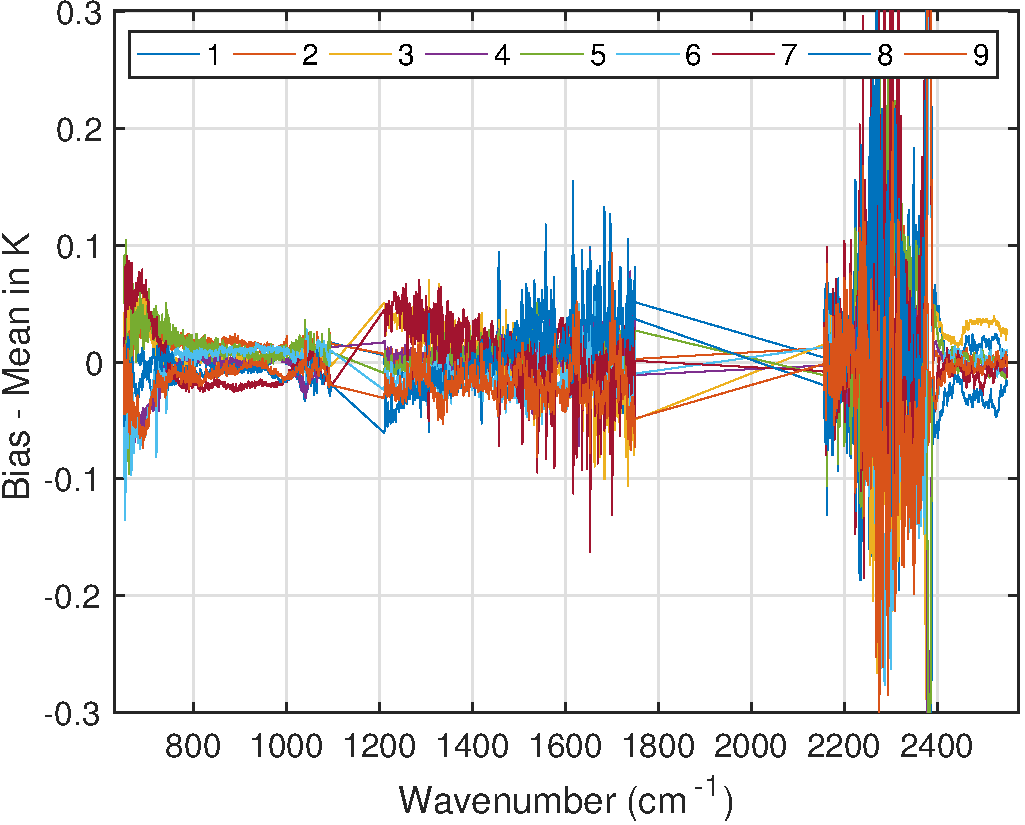
\includegraphics[width=\linewidth]{./testfig.pdf}
        \end{center}
      \end{block}
    \end{column}
  \end{columns}

  We could also adjust SNPP and N2O Neon to be identical for reprocessing.
\end{frame}
% ---------------------------------------------------------------------
\begin{frame}[label={sec:org1a9a034}]{Just bullets}
  \begin{itemize}
  \item We generally only examine near-nadir FORs (15 / 16) in detail.

  \item Users, of course, use all FORs

  \item Examine them here for (a) clear, (b) all-scenes, especially with regard to inter-FOV differences.
  \end{itemize}
\end{frame}
% ---------------------------------------------------------------------
\begin{frame}[label={sec:orgb987c5f}]{Two graphs side-by-side}
  \begin{columns}
    \begin{column}{0.55\columnwidth}
      \begin{block}{Raw Clear FOV BT diffs}
        \begin{center}
          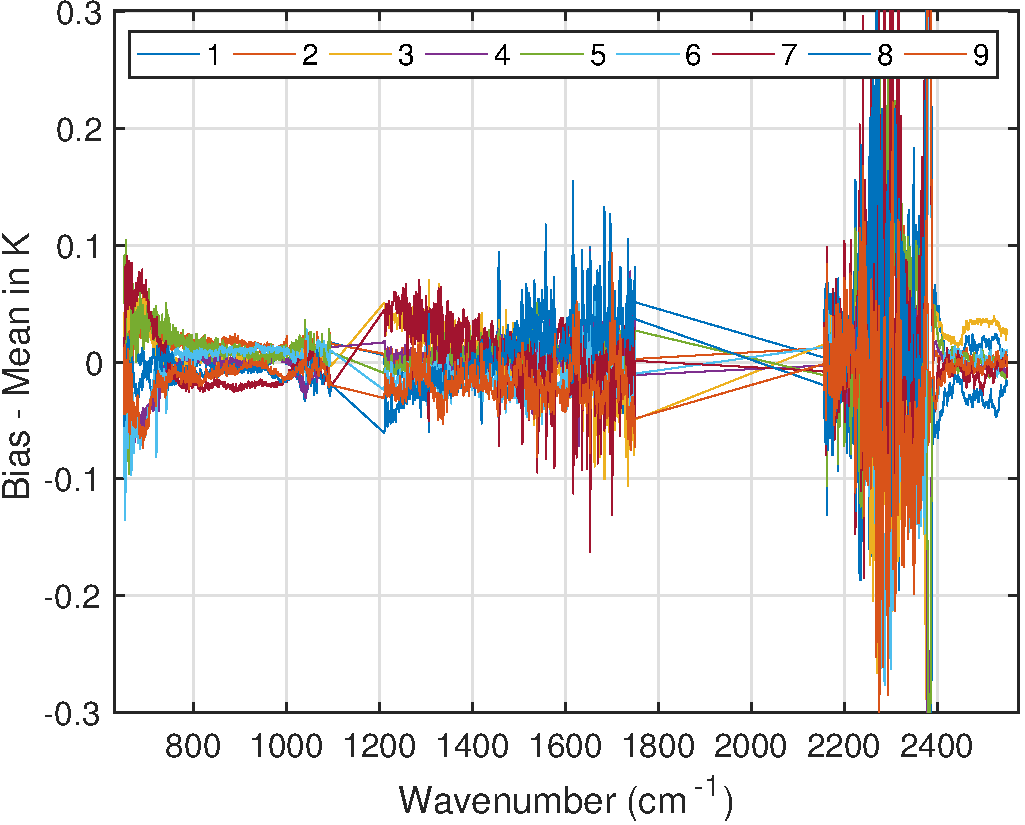
\includegraphics[width=\linewidth]{./testfig.pdf}
        \end{center}
      \end{block}
    \end{column}

    \begin{column}{0.55\columnwidth}
      \begin{block}{NWP Bias Clear FOV BT diffs}
        \begin{center}
          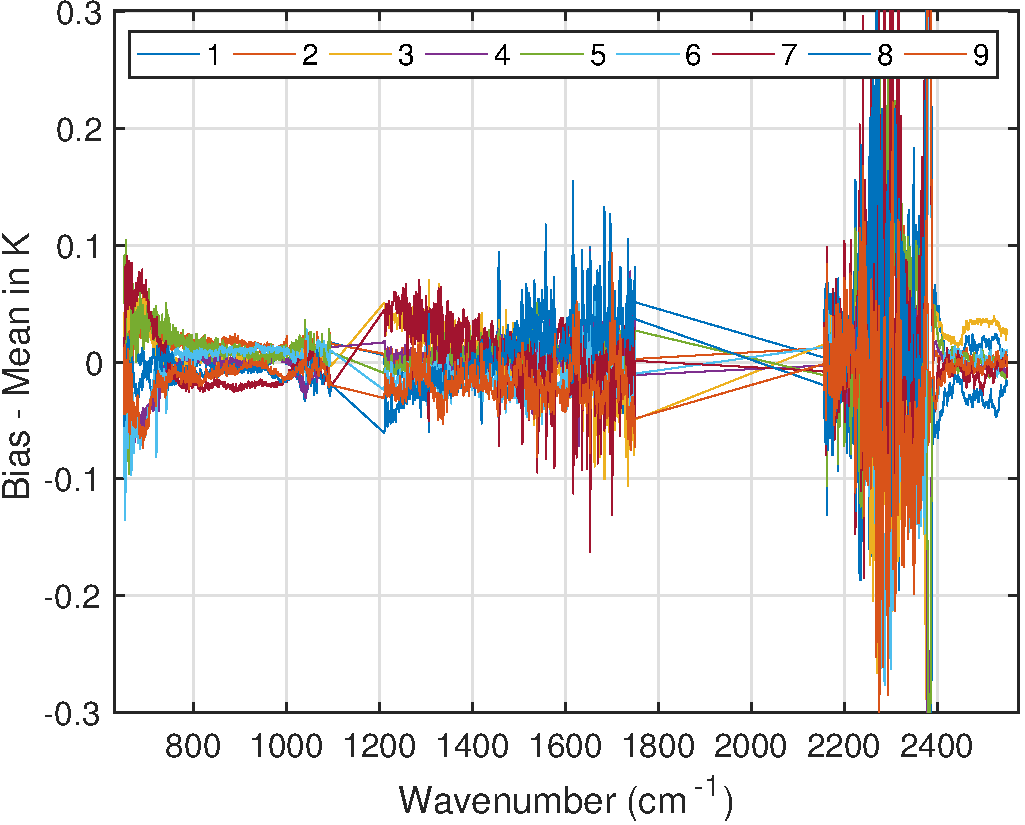
\includegraphics[width=\linewidth]{./testfig.pdf}
        \end{center}
      \end{block}
    \end{column}
  \end{columns}

  Although clear scenes contain all FOVs, there are 3-4X more near nadir than at extreme scan angles.
\end{frame}
% ---------------------------------------------------------------------
\begin{frame}[label={sec:org4279c0f}]{Two graphs top, one centered bottom}
  \vspace{-0.35in}

  \begin{columns}
    \begin{column}{0.5\columnwidth}
      \begin{block}{\footnotesize Secant Diffs with FOR}
        \vspace{-0.05in}
        \vspace{-0.05in}
        \begin{center}
          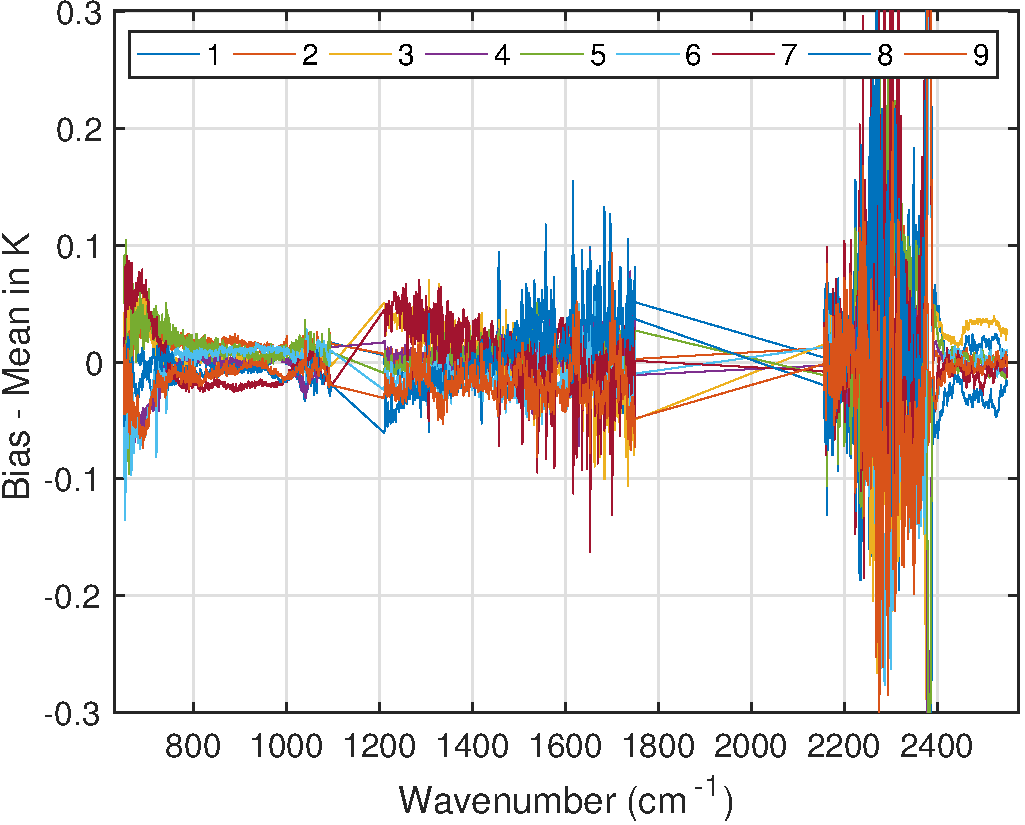
\includegraphics[width=0.85\linewidth]{./testfig.pdf}
        \end{center}
      \end{block}
    \end{column}

    \begin{column}{0.5\columnwidth}
      \begin{block}{\footnotesize Mean Secant Diffs}
        \vspace{-0.05in}
        \vspace{-0.05in}
        \begin{center}
          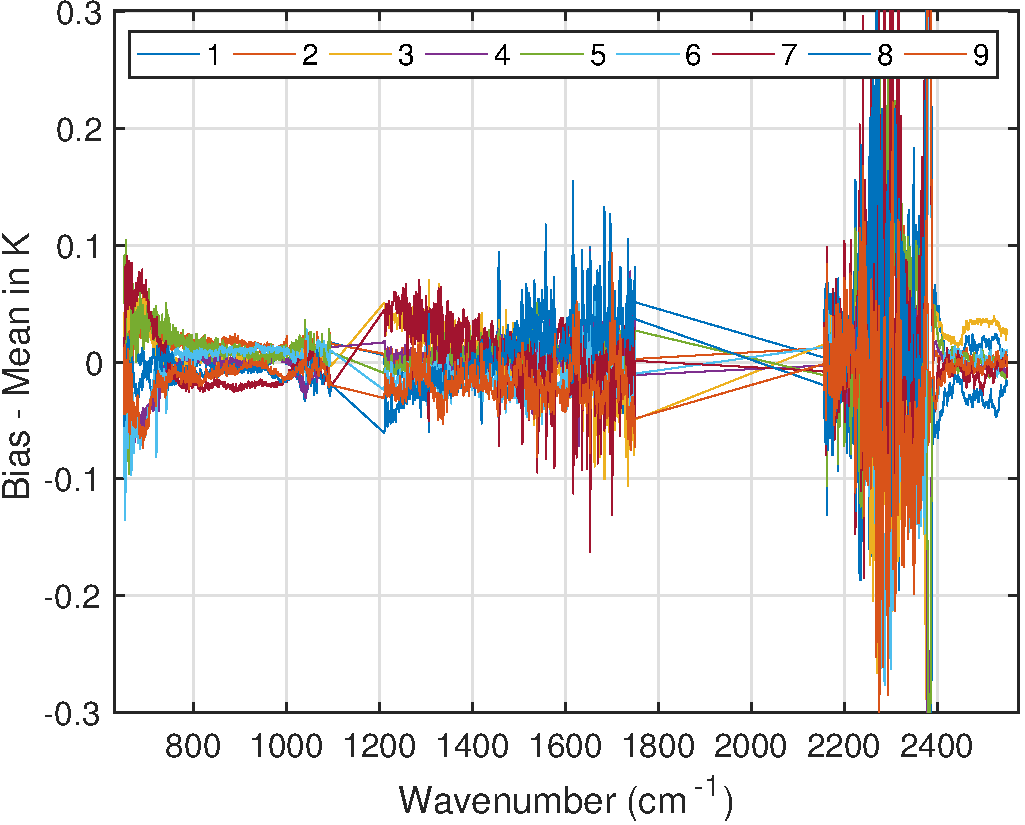
\includegraphics[width=0.85\linewidth]{./testfig.pdf}
        \end{center}
      \end{block}
    \end{column}
  \end{columns}

  \vspace{-0.25in}
  \begin{columns}
    \begin{column}{0.5\columnwidth}
      \begin{block}{\footnotesize Example: FOV9 Secant Corrections}
        \vspace{-0.05in}
        \vspace{-0.05in}
        \begin{center}
          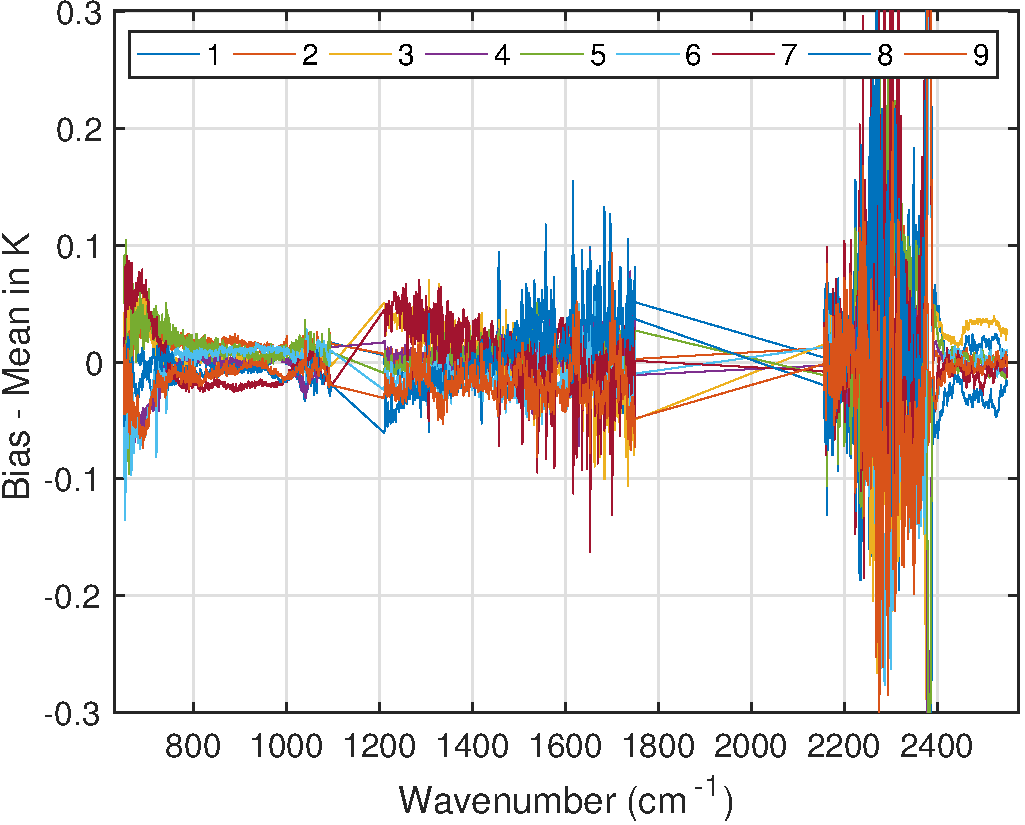
\includegraphics[width=0.85\linewidth]{./testfig.pdf}
        \end{center}
      \end{block}
    \end{column}
  \end{columns}
\end{frame}
% ---------------------------------------------------------------------
\begin{frame}[label={sec:orgb65959b}]{Text full width top, bottom graph left, text right}
  \vspace{-0.1in}
  \begin{itemize}
  \item "Best?" intercalibration of SNPP and N2O is from AIRS SNO double diffs.
  \item AIRS will likely not be up, or operating properly, for J2
  \item Is IASI good enough?
  \item Or, can we use statistical sampling (more later on this)
  \end{itemize}

  \vspace{-0.2in}

  \begin{columns}
    \begin{column}{0.55\columnwidth}
      \begin{block}{\footnotesize Latitude Sampling}
        \vspace{-0.1in}
        \begin{center}
          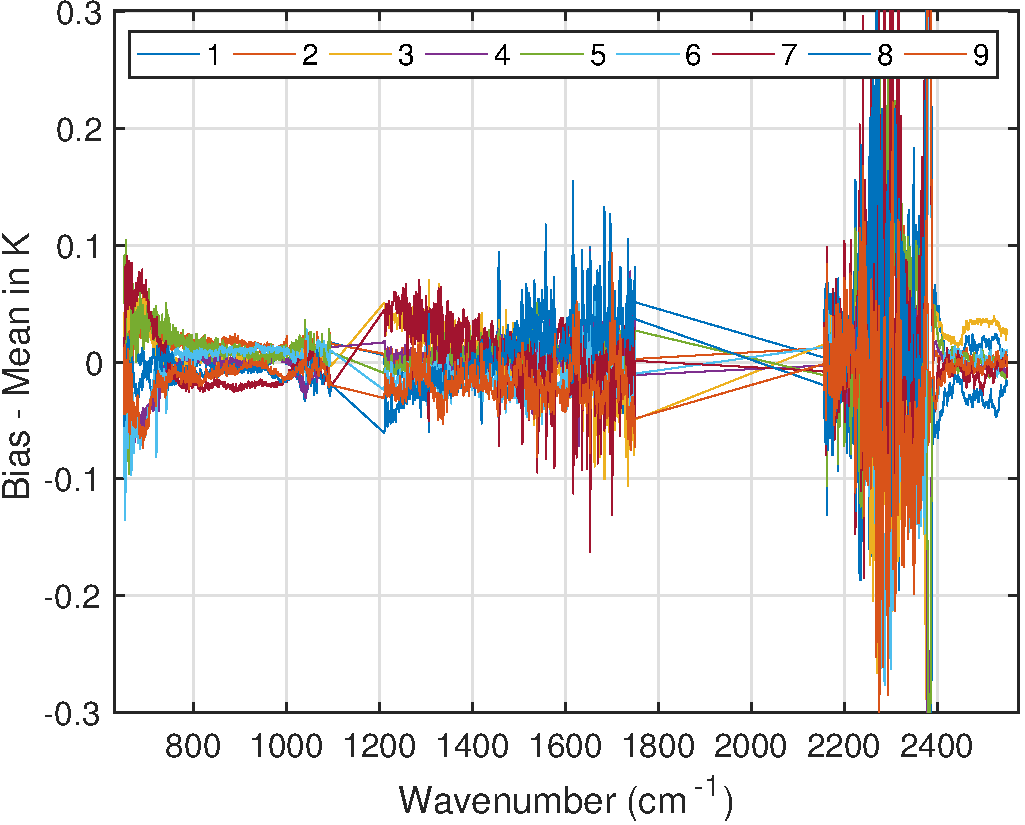
\includegraphics[width=\linewidth]{./testfig.pdf}
        \end{center}
      \end{block}
    \end{column}


    \begin{column}{0.55\columnwidth}
      \begin{block}{\footnotesize}
        \small
        Although scene type sampling is very different for AIRS and IASI, results are fairly similar.  Later will compare with area weighted sampling (for 900 \wn region only).
      \end{block}
    \end{column}
  \end{columns}
\end{frame}
% ---------------------------------------------------------------------
\begin{frame}[label={sec:org791e503}]{Two graphs top, graph bottom left, text bottom right}
  \vspace{-0.3in}
  \begin{columns}
    \begin{column}{0.55\columnwidth}
      \begin{block}{\footnotesize N2O - AIRS}
        \vspace{-0.05in}
        \vspace{-0.05in}
        \begin{center}
          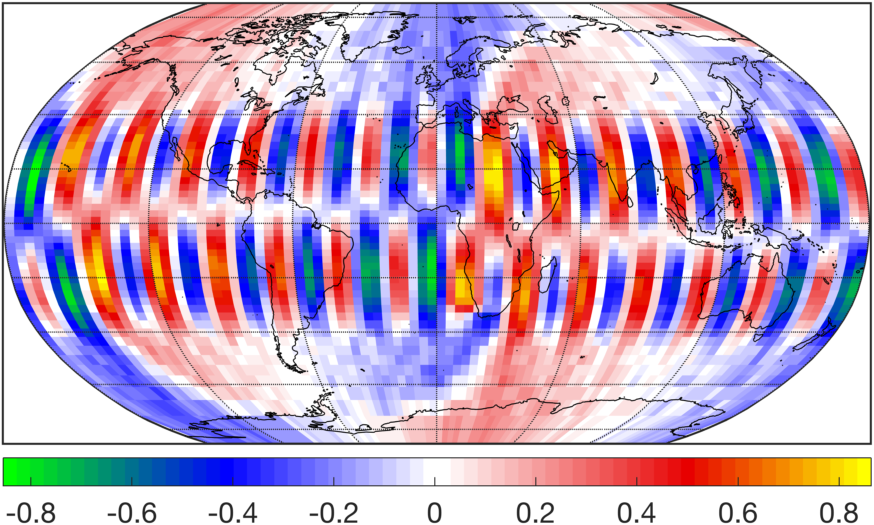
\includegraphics[width=0.95\linewidth]{./testfig.png}
        \end{center}
      \end{block}
    \end{column}

    \begin{column}{0.55\columnwidth}
      \begin{block}{\footnotesize SNPP - AIRS}
        \vspace{-0.05in}
        \vspace{-0.05in}
        \begin{center}
          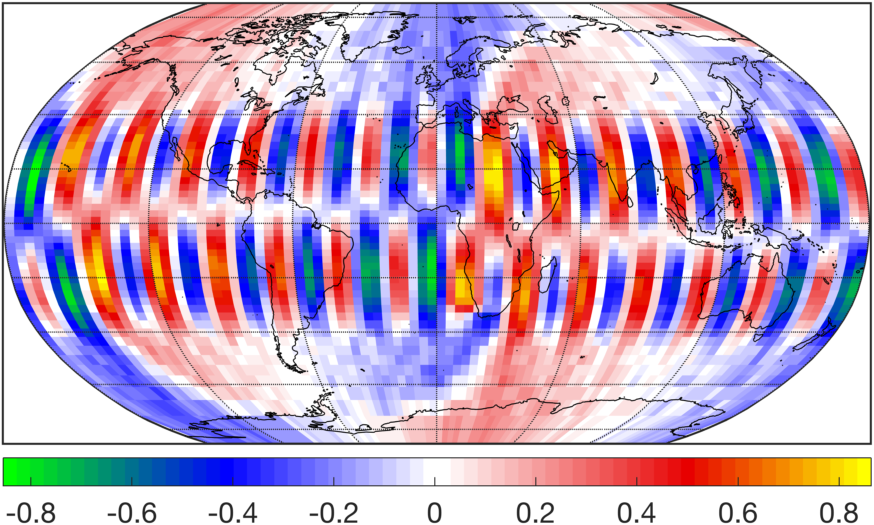
\includegraphics[width=0.95\linewidth]{./testfig.png}
        \end{center}
      \end{block}
    \end{column}
  \end{columns}

  \vspace{-0.1in}
  \begin{columns}
    \begin{column}{0.55\columnwidth}
      \begin{block}{\footnotesize N2O minus SNPP (32\% more variability)}
        \vspace{-0.05in}
        \vspace{-0.05in}
        \begin{center}
          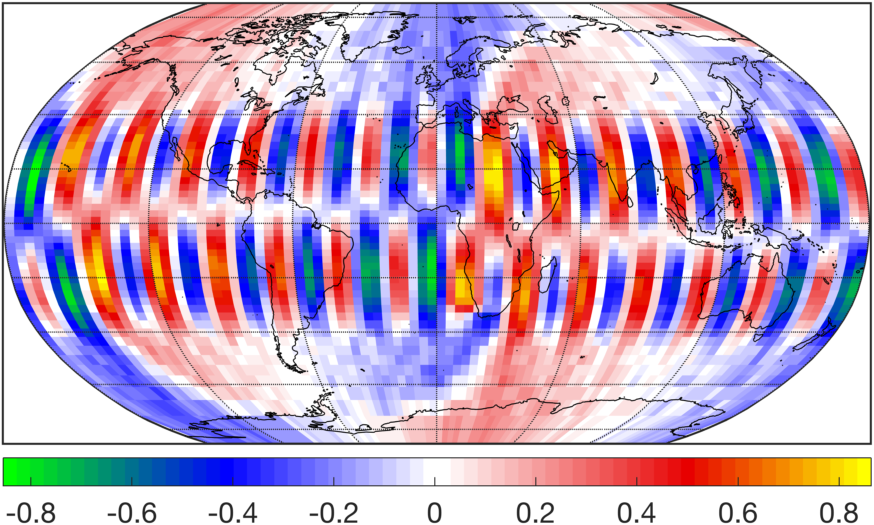
\includegraphics[width=0.95\linewidth]{./testfig.png}
        \end{center}
      \end{block}
    \end{column}

    \begin{column}{0.55\columnwidth}
      \begin{block}{}
        \vspace{-0.1in}
        \begin{itemize}
        \item N2O minus SNPP more variable!
        \item Due to larger time differences!
        \item AIRS SNO: 0.021 K  (0.05K unc?)
        \item IASI SNO: 0.010 K  (0.05K unc?)
        \item Global all FOR statistical differences: 0.013 K
        \end{itemize}
      \end{block}
    \end{column}
  \end{columns}
\end{frame}
% ---------------------------------------------------------------------
% ---------------------------------------------------------------------
\end{document}
% ---------------------------------------------------------------------
% ---------------------------------------------------------------------